%%%%%%%%%%% INCLUSÃO DE PACOTES %%%%%%%%%%%%%%%%
% Classe Base do Documento: Artigo
\documentclass [12pt]{article}
% Layout do Papel
\usepackage{Layout/Layout_Documento}
% Case não funcione, verificar o diretório do arquivo 'Layout_Documento.sty'
%\usepackage{lipsum}
%%%%%%%%%%% FIM INCLUSÃO DE PACOTES %%%%%%%%%%%

%%%%%%%%%%% INFORMAÇÕES BÁSICAS %%%%%%%%%%%%%%%
\title {Projeto Final BD}
%%%%%%%%%%% FIM INFORMAÇÕES BÁSICAS %%%%%%%%%%%

\begin{document}
	\inserirTitulo
	
	\section{Introdução}
		\label{sec:intro}
	Quando há requisito de eficiência nas organizações, tanto com fins lucrativos ou não, é importante que haja conhecimento sobre os dados que transitam por tal organização. Tais dados devem ser trabalhados de modo a se adquirir informações úteis para um bom planejamento, do gerencial ao estratégico.
	
	É possível armazenar tais dados em memória simples de um computador, sendo esta um HD, e realizar todas as operações sobre tais dados; mas há o caso de que, cada vez mais, a massa de dados vem aumentado. Tal aumento exige um gerenciamento adequado, promovido pelos~\emph{Sistemas Gerenciadores de Banco de Dados} (\emph{SGBDs}).
	
	Primeiramente, é preciso compreender o que seria um~\emph{banco de dados} (BD): pode ser visto como o equivalente eletrônico de um armário de arquivamento, uma vez que é a coleção de dados persistentes utilizadas pelos sistemas de aplicação de uma empresa. Dessa forma, um SGBD é responsável pelo gerenciamento dessas coleções, garantindo integridade, segurança e outras características.

	Os dados podem ser extraídos de qualquer fonte, mas, para este trabalho, será utilizada a~\emph{INDA} (\emph{Infraestrutura Nacional de Dados Abertos}); visto que são dados que estão à disposição livremente a todos, mas apenas alguns a acessam. Dessa forma, ao se trabalhar com tais dados e gerar informações consideráveis estaríamos exercendo a nossa cidadania, buscando discrepâncias entre os dados e apontando algumas irregularidades.
	
	Como escopo, foi escolhido os dados sobre~\textbf{Diárias e passagens}~(Tais dados estão disponível~\emph{online}: \url{http://www.portaltransparencia.gov.br/}) limitados ao período: $jan/2015$ a $jun/2015$, visando responder os seguintes questionamentos:
	
	\begin{enumerate}
		\item Qual o gasto total em cada mês?
		\item Quais os órgãos que mais gastaram?
		\item Quais os programas que mais gastaram?
		\item Quais os servidores que mais gastaram?
		\item Quais as funções que mais gastaram?
	\end{enumerate}

	\section{Diagrama Entidade Relacionamento (DER)}
		\label{sec:DER}
	Um DER constitui uma forma de representação gráfica para os conceitos atribuídos ao~\emph{Modelo Entidade Relacionamento} (MER), sendo este um modelo de dados conceitual de auto nível, visto que está centrado na percepção dos usuários sobre os dados, não importando a maneira na qual os dados serão armazenados. Dessa forma, entendisse DER como representação visual sobre os dados que serão tratados no BD.
		
	Como os dados fornecidos vem em forma de planilhas, foi preciso realizar uma leitura e uma interpretação dos mesmos, tentando identificar o que veriam a ser as entidades e os relacionamentos para o nosso BD. Dessa forma, obteve-se a Figura~\ref{fig:DERgerado} como resutaldo do estudo realizado.
	
	\begin{figure}[h]
		\centering
		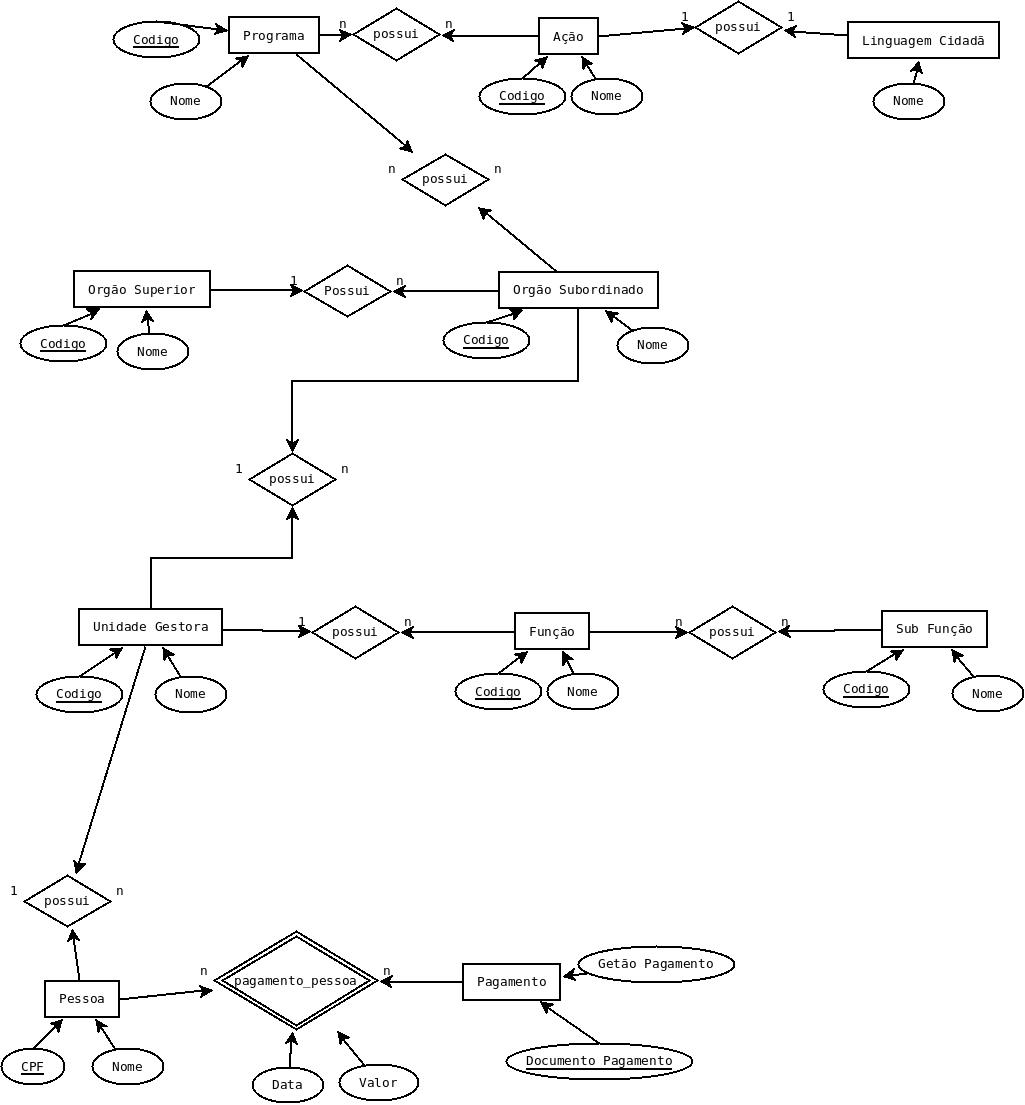
\includegraphics[width=1\textwidth]{Imagens/DER}
		\caption{DER gerado a partir das tabelas e nossa interpretação.}
		\label{fig:DERgerado}
	\end{figure}
	
	
	\section{Modelo Relacional (MR)}
		\label{sec:MR}
	Um MR representa os dados num BD como uma coleção de relações, denominadas de tabelas. Essa coleção será implantada no SGBD, ou seja, o MR representa a construção física do BD. Por isso é desenvolvido a partir do DER e, no escopo deste trabalho, tem-se a Figura~\ref{fig:MRgerado} como resultado.
	
	\begin{figure}[h]
		\centering
		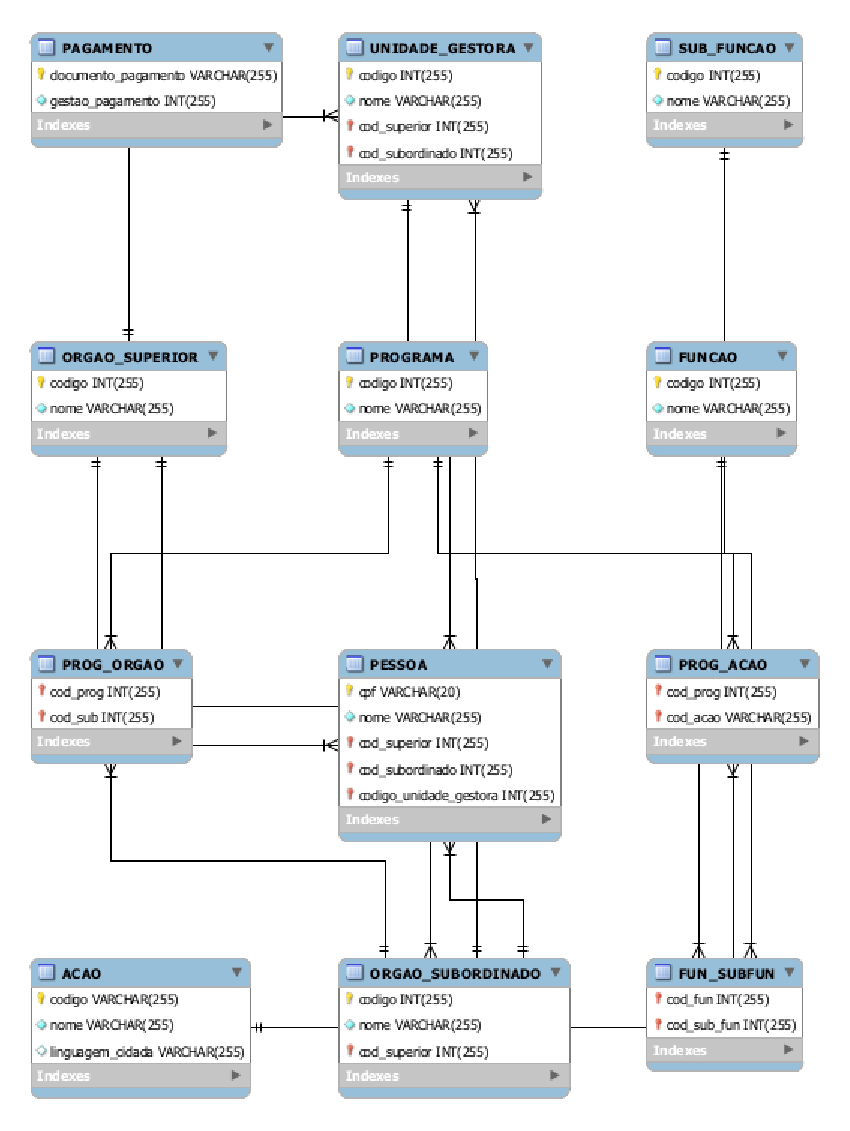
\includegraphics[width=.8\textwidth]{Imagens/MR}
		\caption{MR gerado a partir do DER.}
		\label{fig:MRgerado}
	\end{figure}
	
	\section{Avaliação das formas normais}
		\label{sec:FormaisNormais}
		
	\section{Criação do BD}
		\label{sec:BDcreate}
		
	\section{Processo de ETL}
		\label{sec:ETL}
		
	\section{Persistência e Visualização}
		\label{sec:Per&Vis}
\end{document}
